\documentclass[]{sigplan-proc}
\usepackage{graphicx}
\usepackage{epstopdf}
\usepackage{url}
\usepackage{listings}
\usepackage[colorlinks,urlcolor=blue]{hyperref}
\renewcommand{\topfraction}{0.85}
\renewcommand{\textfraction}{0.1}

\conferenceinfo{TBD}{TBD}
\CopyrightYear{2012}
\crdata{}

\begin{document}

\title{ A Study of Lustre Networking Over a 100 Gigabit Wide Area Network with 50 milliseconds of Latency}

\numberofauthors{3}
\author{
\alignauthor Scott Michael\\
	\affaddr{Indiana University}\\
	\affaddr{Bloomington, IN 47408}\\
	\email{scamicha@iu.edu}
\alignauthor Liang Zhen\\
        \affaddr{Whamcloud Inc.}\\
        \affaddr{Danville, CA 94526}\\
        \email{liang@whamcloud.com}
\alignauthor Robert Henschel\\
        \affaddr{Indiana University}\\
        \affaddr{Bloomington, IN 47408}\\
        \email{henschel@iu.edu}
\and
\alignauthor Stephen Simms\\
	\affaddr{Indiana University}\\
	\affaddr{Bloomington, IN 47408}\\
	\email{ssimms@indiana.edu}
\alignauthor Eric Barton\\
        \affaddr{Whamcloud Inc.}\\
        \affaddr{Danville, CA 94526}\\
        \email{eeb@whamcloud.com}
\alignauthor Matthew Link\\
	\affaddr{Indiana University}\\
	\affaddr{Bloomington, IN 47408}\\
	\email{mrlink@indiana.edu}		
}

\maketitle

\begin{abstract}

  As part of the SCinet Research Sandbox at the Supercomputing 2011 conference, Indiana University utilized a
  dedicated 100 Gbps wide area network (WAN) link spanning more than 3,500 km (2,175 mi) to demonstrate the
  capabilities of the Lustre high performance parallel file system in a high bandwidth, high latency WAN
  environment. This demonstration functioned as a proof of concept and provided an opportunity to study
  Lustre's performance over a 100 Gbps WAN. To characterize the performance of the network and file system a
  series of benchmarks and tests were undertaken. These included low level iperf network tests, Lustre
  networking (LNET) tests, file system tests with the IOR benchmark, and a suite of real-world applications reading
  and writing to the file system. All of the tests and benchmarks were run over a the WAN link with a latency
  of 50.5 ms. In this article we describe the configuration and constraints of the demonstration and focuses in
  on the key findings and discoveries made regarding the Lustre networking layer for this extremely high
  bandwidth and high latency connection. Of particular interest is the relationship between the {\tt peer\_credits}
  and {\tt max\_rpcs\_in\_flight} settings when considering LNET performance.

\end{abstract}

\category{H.3.4}{Information Storage and Retrieval}{Systems and Software}[Distributed systems, Performance evaluation (efficiency and effectiveness)]
\category{C.2.2}{Computer-\linebreak Communication Networks}{Network Protocols}[Protocol architecture (OSI model),
Routing protocols]

\terms{Algorithms, Performance}

\keywords{WAN file systems, Lustre, 100 Gbit Networking}

\section{Introduction}\label{sec:intro}

The SCinet Research Sandbox (SRS) at the Supercomputing 2011 (SC11) conference encourages institutions to
showcase new and innovative technologies in the area of networking. For the demonstration SCinet, in
collaboration with ESnet and Internet2, provided SRS participants with a 100 Gbps network connection from
the SC11 show floor to the Internet2 backbone. This link provided an end-to-end connection from the IU booth
on the SC11 show floor to the IU Data Center in Indianapolis, Indiana. 

The overall goal of the IU entry into the SRS was to demonstrate the use of a Lustre file system in scientific
applications over the 100 Gbps wide area network (WAN) spanning from Seattle, Washington to Indianapolis,
Indiana, a distance in excess of 3,500 km (2,175 mi). A diagram of the network and routing points is given in
figure \ref{fig:network}. Such a use case is of obvious intrest for geographically distributed workflows; for
example, when data sources, such as remote sensors are in locations very distant from computational resources
used to analyze the data \cite{henschel2010}. Though the overall demonstration was ultimately successful, IU
achieved the highest reported throughput (6.2 GB/s) with scientific applications running across the WAN, the
focus of this article is the performance of and lessons learned about the Lustre networking layer, LNET.

\begin{figure*}[t]
\begin{center}
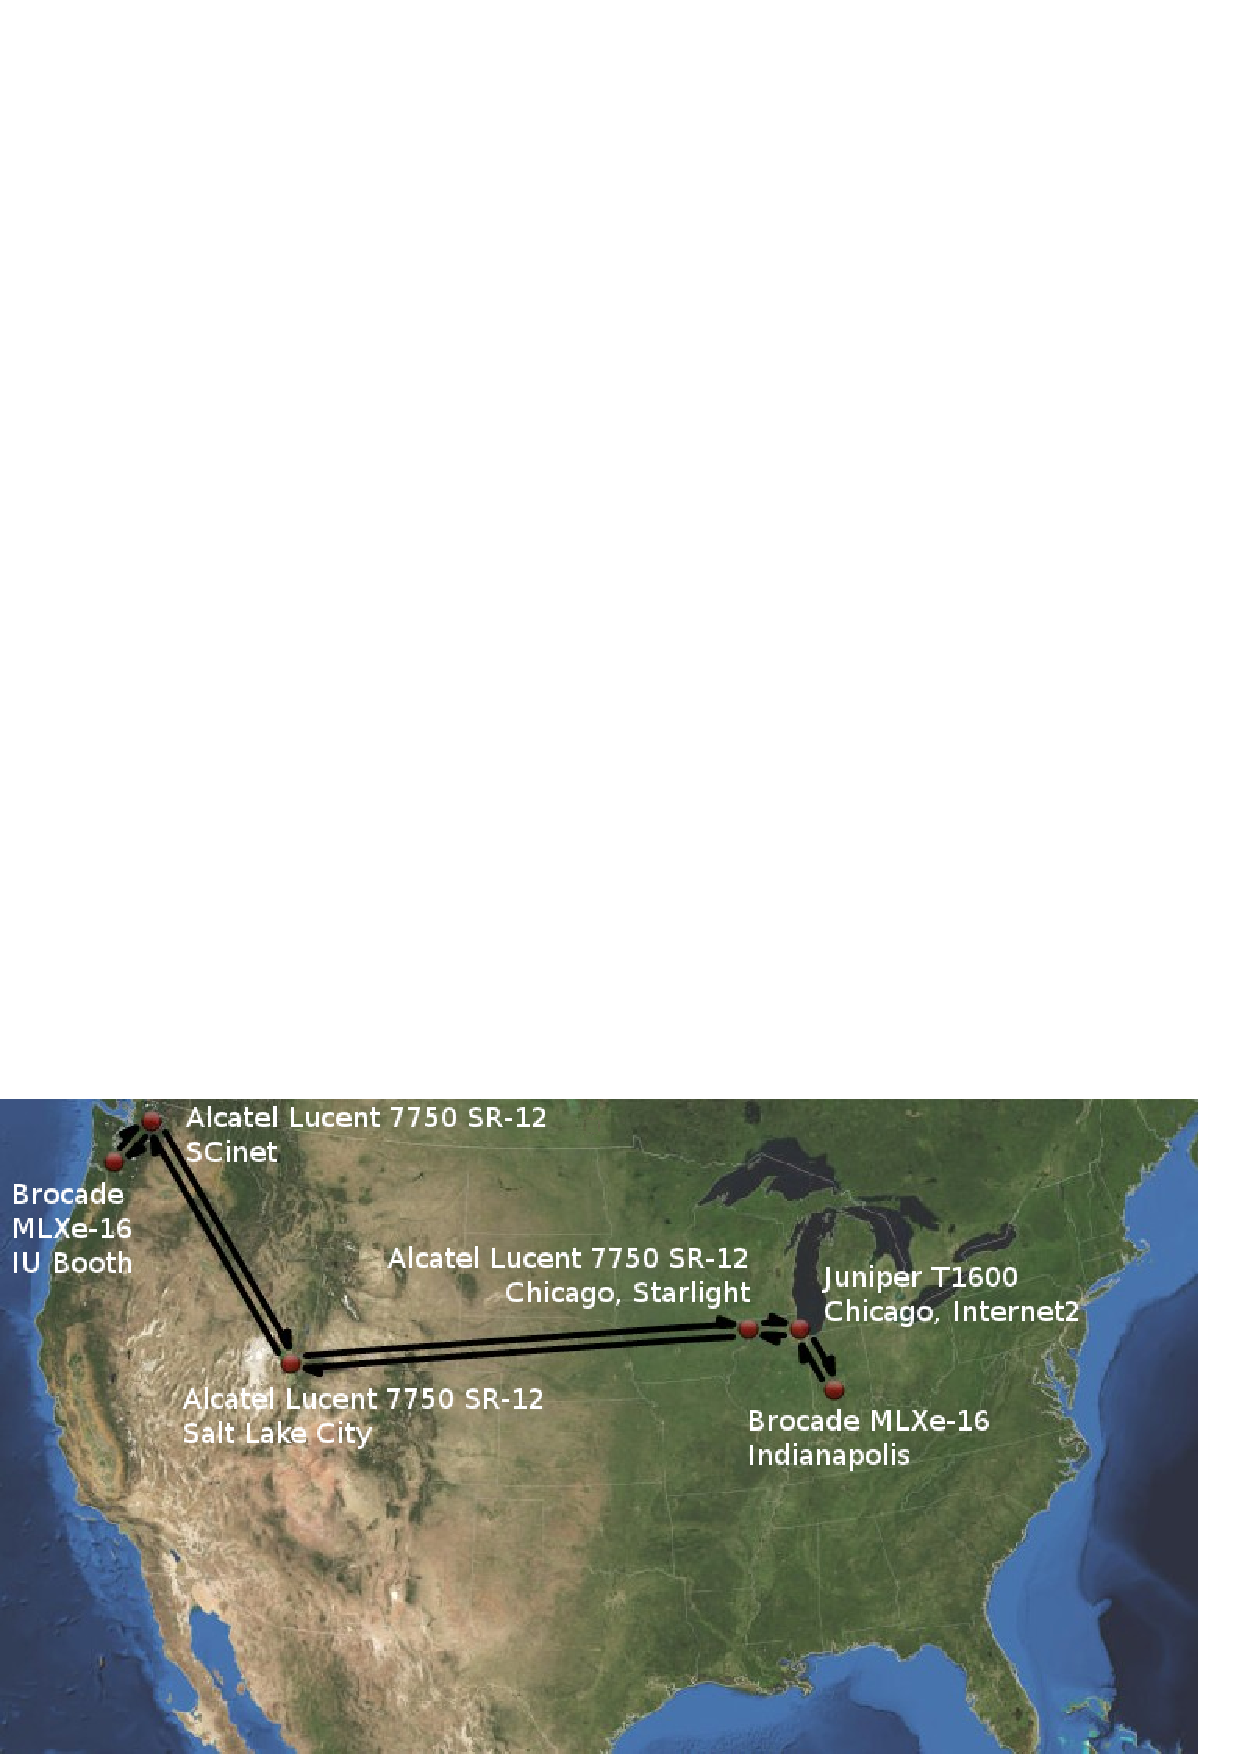
\includegraphics[width=0.80\textwidth]{figures/network.png}
\caption{Networking diagram for SRS demonstration. Routing points are labeled in the diagram.}
\label{fig:network}
\end{center}
\end{figure*}

Access to the 100 Gbps WAN was facilitated and coordinated by SCinet. Each participant was given time slots
for exclusive use of the network. The slots were evenly distributed from Saturday, November 12th to Thursday,
November 17th. In total, IU was provided nine test slots for a combined 16 hours. All testing that required
access to the network links had to be performed during those times, from setting up the actual end to end
network connectivity to performing file system and application tests. In addition, we were provided five
demonstration slots for a total of four hours. Those time slots were used to showcase the capabilities of the
system in the IU booth. All results described in this article were obtained in the 20 hours of demonstration
and test time.

The fact that this study was performed in such a limited timeframe influenced the measurements we were able to
take. In addition to the fact that the time allotted to IU was fairly short, the initial connection of the 100
Gbps link required some fine tuning of the routing elements between Seattle and Indianapolis to achieve an
eventual uni-directional peak throughput of 96 Gbps on the TCP layer \cite{henschel2012}. Although some of the
network issues were eventually resolved, the network was quite variable throughout the SC11 conference and we
were never able to achieve full bi-directional throughput. In addition, the network phase of the
troubleshooting consumed nearly half of the time allocated to IU, leaving approximately 10 hours for
troubleshooting and gathering data on LNET, file system benchmarks, and the performance of scientific
applications.

This paper is structured as follows: Section \ref{sec:LNET} gives a brief technical overview of the LNET layer
of Lustre with particular attention paid to remote procedure calls (RPCs) and peer credits. Section
\ref{sec:usecase} describes in detail the SRS use case, including the hardware setup that was used for the SRS
demonstration and the particulars of the Lustre installation and software tools used. Section
\ref{sec:results} describes the results obtained from measurements of the Lustre networking layer. In section
\ref{sec:discussion} we offer some hypotheses explaining the results and compare to previous work. A summary and conclusion follows in section \ref{sec:conclusion}.

\section{The Lustre Networking Protocol}\label{sec:LNET}

The Lustre networking protocol (LNET) sits above the underlying network stack (e.g. TCP, IB, etc.) and
mediates the communication between Lustre components such as clients, servers, and metadata servers. 

{\bf COULD A MORE ACCOMPLISHED LNET EXPERT LIKE SIMMS, LIANG, OR BARTON ADD SOME MORE HERE?}

\subsection{Lustre Remote Procedure Calls}

The Lustre remote procedure call (RPC) mechanism allows one to send requests, receive and process requests,
perform bulk data transfer, and provide for error recovery. The number of outstanding RPCs that a single
client may submit to a single server is controlled by the Lustre tunable {\tt max\_rpcs\_in\_flight}. This is
a client-side setting and may be set on a per client basis. The default setting of {\tt max\_rpcs\_in\_flight}
= 8 may be suitable for many data center environments where there is relatively low latency between the
storage system and the clients it serves. However, in a WAN environment round-trip times (RTTs) tend to be
much longer and in order to keep the maximum number of RPCs ``on the wire'' the {\tt max\_rpcs\_in\_flight} is
typically increased. Though one might think that raising the ceiling on RPCs should always improve
performance, the potential drawback lies in the fact that a single client can then consume more resources on a
server, and at some point, if {\tt max\_rpcs\_in\_flight} are increased across all clients, the server may
become overwhelmed. It should also be noted that the {\it Lustre Operations Manual} \cite{LustreManual2012}
incorrectly states that the largest value {\tt max\_rpcs\_in\_flight} may take is 32, when, in fact, we tested
values up to and including {\tt max\_rpcs\_in\_flight} = 256.

We are mainly concerned with sends, receives, and bulk transfers because our LNET testing focused on bulk
operations. In Lustre a bulk transfer operation requires one RPCs to complete. The RPC request for a write
from the client to the server works as follows {\bf EXPLANATION FROM BARTON}. So then, the maximum data
transfer rate for a single RPC is equal to the volume of the data transferred, i.e. the block size, divided by
two times the RTT of the network link. Thus the peak throughput for a given number of RPCs is
\begin{equation}
\mathrm{Peak Bandwidth = \frac{RPCs \times BS}{2 \times RTT}},
\label{eq:band}
\end{equation}
where RPCs is the maximum number of RPCs in flight, and BS is the block size of the RPC packets, typically 1
MB. Equation \ref{eq:band} represents a theoretical maximum and does not take into account the physical
limitations of a given network link.

Based on equation \ref{eq:band}, the minimum number of RPCs required to saturate a WAN link with a given
bandwidth delay product (BPD), obeys the following relationship.
\begin{equation}
\mathrm{RPCs > \frac{2\times BDP}{BS},}
\label{eq:rpcs}
\end{equation}
where RPCs is the {\it total} number of RPCs needed, and is a product of the Lustre tunable {\tt
  max\_rpcs\_in\_flight}, number of clients, and number of servers per client (i.e. stripes). BDP is the
bandwidth delay product given by, $\mathrm{link bandwidth \times RTT}$. This relationship has been seen
previously by Simms et al. \cite{simms2007}, but was not stated in this form. For the 100 Gbps link used in
the SRS demonstration, with a 50.5 ms RTT and 1 MB block size, slightly more than 5,000 RPCs are needed.

\subsection{Lustre Peer Credits}

If one uses ksocklnd for the communication between Lustre network devices (LNDs) further tuning parameters
governing the amount of data ``on the wire'' are available within the ksocklnd module. The key parameters in

{\bf THIS NEEDS SOME INTRODUCTION ABOUT WHAT ksocklnd actually is.... Barton, Simms?}

the case of the SRS demonstration, which we present results for in section \ref{sec:results}, were 
{\tt credits} and {\tt peer\_credits}. While the {\tt max\_rpcs\_in\_flight} parameter is applicable at a higher
layer, {\tt credits} and {\tt peer\_credits} control the number of messages that can be concurrently sent over
a LND network interface (NI). The {\tt credits} value determines the maximum number of {\it total} concurrent
sends from a NI, while the {\tt peer\_credits} value determines the maximum number of concurrent sends from a
NI to the same destination, or peer. By default {\tt credits} is set to 64 and {\tt peer\_credits} is set to
8. This means that if a single client stripes files over more than 8 servers using 8 {\tt peer\_credits} it
will exceed the number of allocated {\tt credits}. It should be noted that {\tt credits} and {\tt
  peer\_credits} apply to sends only, while {\tt max\_rpcs\_in\_flight} apply to both sends in
receives. Additionally, {\tt credits} and {\tt peer\_credits} are returned to their pool once the send is
completed and ``on the wire'', while RPCs can be outstanding for a longer period of time as they are not
retired until data hits the Lustre object storage target (OST).Due to these facts, one might expect
transactions to require a greater number of {\tt max\_rpcs\_in\_flight} than {\tt peer\_credits}.
 

\section {The SC11 Example Case}\label{sec:usecase}

As outlined in section \ref{sec:intro}, to showcase the capabilities of Lustre we set up a Lustre
file system and mounted it across the 100 Gbps cross-country WAN. To preform the demonstration we set up a
compute cluster on the show floor in Seattle and one in the IU data center in Indianapolis. We also deployed a
file system at each location. In addition, we installed and configured networking components to connect to the
Internet2/ESnet endpoints. The rest of this section details the hardware, network, Lustre, and other software
set up and configuration that was applied for the demonstration.

\subsection{Hardware}\label{sec:hardware}

Figure \ref{fig:hardwaresetup} shows the final hardware configuration that was used for the SRS demonstration. IBM provided 31 servers that functioned as compute nodes as well as the 16 storage servers that
were attached to the DataDirect Networks (DDN) storage devices. Brocade and Ciena provided the routing
equipment that enabled the network link from the show floor to Indianapolis.

The configurations of the compute cluster, storage, and networking components were identical in both
Indianapolis and Seattle. The central networking component at each endpoint was a Brocade MLXe-16 router that
provided a 100 Gbps Ethernet connection to the Ciena optical terminal managed by Internet2. The core router
also provided a 10 Gbps link to an IBM BNT G8264 OpenFlow enabled switch at each endpoint. The SRS
demonstration comprised a OpenFlow component in addition to the main Lustre 100 Gbps demonstration. However,
we will not discuss the OpenFlow component in this article. The 31 compute servers and 16 Lustre storage
servers were attached directly to the Brocade core router at 10 Gbps using Twinax cables and Brocade 1860
dual-port adapters.

The compute servers were IBM System x iDataPlex dx360 M3 systems, each configured with dual Intel Xeon E5645
6-core 2.40 GHz processors, 24 GB of DDR3 RAM, a Brocade 1860 adapter, and a 250 GB SATA hard drive. The
object storage servers (OSS) were IBM System x iDataPlex dx360 M3 servers each configured with an Intel Xeon
E5645 6-core 2.40 GHz processor, 48 GB of DDR3 RAM, a Brocade 1860 adapter, and a 1 TB SATA hard drive. The
OSS nodes at each site were connected directly to a DDN SFA10000 via 8 Gb Fibre Channel (FC). The metadata
server was identical to the compute servers, except it had 96 GB of RAM and was directly connected to a DDN
EF3015 RAID system that contained twelve 300 GB 15K RPM SAS disk drives for Lustre metadata. Due to space
constraints on the show floor server density was important. The throughput of the DDN SFA10000 allowed us to
use a single storage system for the Lustre OSS nodes at each site.

\begin{figure*}[t]
\begin{center}
\includegraphics[width=0.80\textwidth]{figures/hardware.png}
\caption{Shown here is the hardware configuration used for the SRS demonstration. An IBM iDataPlex cluster and
  Lustre file system were connected to a Brocade 100 Gpbs MLXe-16 router at each endpoint. The IBM routing
  equipment connected to the Brocade routers was used for the OpenFlow component of the demonstration and is
  not discussed in this article. }
\label{fig:hardwaresetup}
\end{center}
\end{figure*}

\subsection{Network}\label{sec:network}

Before shipping equipment to the show floor in Seattle the demonstration configuration was assembled in the IU
machine room for testing.  There we performed tests with the two Brocade MLXe routers connected back to back
with the 100 Gbps connection spanning a few meters.  Local network tests across this connection showed a
latency of 0.24 ms and maximum stable performance of 98 Gbps using TCP iperf \cite{iperf2012}.

The network link that was used for the SRS demonstration provided 100 Gbps connectivity from the IU booth on
the SC11 show floor to the IU Data Center in Indianapolis. In the months preceding the SC11 conference,
Indiana University worked with Internet2 to upgrade the existing link from Chicago to Indianapolis to 100
Gbps. For the SRS demonstration Internet2 and ESnet provided access to the 100 Gbps link from Chicago to Salt
Lake City and on to Seattle. From that point on to the show floor, SCinet was responsible for the network
link. The connection from Salt Lake City to Seattle had been established at 100 Gbps only two weeks prior to
SC11 and had undergone little to no performance testing.

Once the link was established, we measured a 50.5 ms round-trip time (RTT) between the clusters in Seattle and
Indianapolis. Initial TCP iperf tests showed good performance for two parallel streams, each at 10
Gbps. However, when adding more iperf streams to the link, performance dropped and throughput become
unstable. Working with Internet2, ESnet, and SCinet, we were able to tune several parts of the network and
achieve a stable 80 Gbps throughput with TCP iperf. Following all of our modifications, we were able to put a
stable 80 Gbps of TCP iperf traffic on the link by using 8 servers and clients. Unfortunately, adding another
single 10 Gbps stream to either of the connections resulted in congestion and degraded performance. However,
when oversubscribing the link by using all 30 compute nodes on each end, we were able to achieve a peak
throughput of 96 Gbps. Another unfortunate outcome was that the tuning steps yielded a stable connection only
in one direction, from Seattle to Indianapolis. We were never able to achieve similar results in the other
direction, and due to time constraints, we focused our efforts on just one direction.

\lstset{language=Bash, caption=Tuning parameters for the network, label=TuningListing}
\begin{lstlisting}
net.ipv4.tcp_rmem=4096 65536 167772160
net.ipv4.tcp_wmem=4096 65536 167772160
net.core.rmem_max=167772160
net.core.wmem_max=167772160
net.core.netdev_max_backlog=30000
eth2 txqueuelen 10000
eth2 mtu 9000
FlowControl off 
\end{lstlisting}

Listing \ref{TuningListing} shows the network tuning parameters that were set on all nodes. We increased the maximum TCP buffer to 167 MB and increased the sending and receiving queues to 10000 and 30000. In addtion, we enabled MTU 9000 and configured all nodes to use the \texttt{tcp\_bic} network stack. Flow control was disabled on the network adapters and the routers.

\subsection{Software and Lustre Configuration}

All of the clients and Lustre servers ran RedHat Enterprise Linux version XXXX. The Lustre servers used a
patched kernel with Lustre version XXX, while the clients used the patchless client version of Lustre with
version number XXX. Tests were conducted with the LNET self-test module that is part of the Lustre modules
toolkit. The LNET self-test scripts used to collect measurements for the SRS demonstration are available on
Github.com \cite{lstgithub2011}.

{\bf SIMMS NEED SOME ADDITIONAL STUFF HERE. MAYBE SHOULD OUTLINE THE OST CONFIG HERE?}

\section{Results}\label{sec:results}

In this section we present the results collected from the system using the LNET self-test module and self-test
scripts that we have made available \cite{lstgithub2011}. The first tests we conducted were on the system that
was built in the IU data center with the two systems connected back to back. As reported in section
\ref{sec:network}, we were able to achieve 98 Gbps with iperf TCP tests. Performing an LNET self-test from 30
clients to 16 servers yielded a throughput over 90 Gbps, which was in keeping with previous experiments
\cite{kluge2012}.

After deploying the systems on the SC11 show floor and extensive network tuning to get a stable 80 Gbps TCP
connection, we performed a series of LNET self-test measurements over the WAN. We varied the number of clients
and servers, and the LNET concurrency. The concurrency parameter in the LNET self-test, although not
identical, is analogous to the {\tt max\_rpcs\_in\_flight} setting. The difference lies in the fact that {\tt
  max\_rpcs\_in\_flight} applies to a layer above LNET and so knows about things like OSTs, for example. But,
for all intents and purposes, at the LNET level concurrency and {\tt max\_rpcs\_in\_flight} are
equivalent. For the duration of this article we will use the terms LNET concurrency and RPCs in flight
interchangeably.  

\begin{figure}
\centering
\includegraphics[width=0.50\textwidth]{figures/default_pc_plot.eps}
\caption{Results of LNET self-test for 1, 2, and 4 clients using the default settings of 8 and 64 for {\tt
    peer\_credits} and {\tt credits}, respectively.}
\label{fig:default}
\end{figure}

Our initial tests for a single server, using the default {\tt peer\_credits} and {\tt credits} values, are
shown in figure \ref{fig:default}. Plotted is the throughput reported by LNET self-test for RPCs ranging from
1 to 256. Results are shown for 1, 2, and 4 clients communicating with a single server. Each self-test run for
a given number of RPCs and clients was run for 20 seconds before the measurement was taken so as not to be
contaminated by the initial TCP ramp up phase. All self-test results reported here used a 1:1 distribution,
meaning that each client maps to one, and only one, server. The servers are handed out to the clients in a
round robin fashion. This fact is not important for the single server tests, but for the whole system (30
clients and 16 servers) most servers connected to two clients while two servers had only a single client.

Remember that each client and server was equipped with a 10 Gbps network interface, meaning that the
theoretical peak throughput of the hardware was 1250 MB/s. Although, as we expected, we saw a greater
throughput with a larger number of clients, the absolute numbers were far below what we had initially
expected.

\begin{figure}
\centering
\includegraphics[width=0.50\textwidth]{figures/32pc_plot.eps}
\caption{Results of LNET self-test for 1, 2, and 4 clients using the settings of 32 and 1024 for {\tt
    peer\_credits} and {\tt credits}, respectively.}
\label{fig:32pc}
\end{figure}

Following the rather low performance numbers seen in our initial tests we increased the {\tt credits} and {\tt
  peer\_credits} values from their defaults to 1024 and 32, respectively. Though {\tt peer\_credits} were only
increased by a factor of four, {\tt credits} were increased much more dramatically as we intended to stripe
files more than eight ways in the file system benchmarks. Figure \ref{fig:32pc} shows the results for 1, 2,
and 4 clients connecting to a single server for a range of RPCs after the credits had been increased. Clearly,
the results are improved over the previous settings, but even with 4 clients the throughput was barely over
50\% of the theoretical peak.  

\begin{figure}
\centering
\includegraphics[width=0.50\textwidth]{figures/64pc_plot.eps}
\caption{Results of LNET self-test for 1, 2, and 4 clients using the settings of 64 and 2048 for {\tt
    peer\_credits} and {\tt credits}, respectively.}
\label{fig:64pc}
\end{figure}

Finally, we increased {\tt credits} and {\tt peer\_credits} to 2048 and 64, respectively. The results from
these tests are shown in figure \ref{fig:64pc}. In this case we were able to achieve a peak of 1092 MB/s or
87\% of the theoretical peak. We assume that the 2 and 4 client cases ran into some sort of TCP congestion for
128 and more RPCs, which would account for the decreased performance for those RPC values.

In order to explore the seemingly profound effect that the two credits settings have on throughput for RPCs
greater than 8, we took a closer look at the simplest case: a single client and a single server. The single
client results from figures \ref{fig:default}, \ref{fig:32pc}, and \ref{fig:64pc} are plotted side-by-side in
figure \ref{fig:singleserver}. Based on equation \ref{eq:band} we calculated the maximum bandwidth that can
be achieved given the {\tt max\_rpcs\_in\_flight}, the RTT of the link, and the block size.
This peak bandwidth is also included in figure \ref{fig:singleserver} as a function of RPCs. One can see that
for this simple case, where communication between client and server is most deterministic, the bandwidth
achieved tracks the theoretical peak for RPCs up to the number of {\tt peer\_credits}. For RPC values greater
than the number of {\tt peer\_credits} performance can continue to improve, but the rate of improvement
rapidly diverges from the theoretical peak. 

\begin{figure}
\centering
\includegraphics[width=0.50\textwidth]{figures/ss_plot.eps}
\caption{A comparison of single client, single server results of LNET self-test for 8, 32, and 64 {\tt
    peer\_credits}. The values of {\tt credits} were set according to the {\tt peer\_credit} values. Also
  plotted is the theoretical peak throughput based on the number of RPCs as derived from equation \ref{eq:band}.}
\label{fig:singleserver}
\end{figure}

Finally, we look at the effect that {\tt credits} and {\tt peer\_credits} have on the whole system. Figure
\ref{fig:allserver} shows the throughput values measured for 30 clients and 16 servers. As mentioned earlier,
the self-tests were run in a 1:1 distribution. So, for these measurements 14 of the servers were connected to
2 clients, while 2 servers only had a single client. One can notice a trend similar to those seen in the
previous figures. Namely, as {\tt peer\_credits} are increased, the aggregate bandwidth achieved increases for
higher RPC values. However, with the full 30 clients and 16 servers we were unable to saturate the 100 Gbps
link for any combination of {\tt max\_rpcs\_in\_flight}, {\tt credits}, and {\tt peer\_credits} we tested. Since the {\tt max\_rpcs\_in\_flight} parameter is set on a per client basis, one can
calculate the theoretical peak throughput by multiplying equation \ref{eq:band} by the number of clients; in
this case 30. Theoretical peak values are included in as a dashed line in figure \ref{fig:allserver}, and are
based solely on the total number of RPCs without taking the physical limitation of the link into
account. Given that we were able to achieve the theoretical throughput for a single client and server, it is
difficult to say why the throughput values were so much smaller than the peak theoretical values for RPCs
greater than 8, even when {\tt peer\_credit} were set to 64. We hypothesize that the culprit could be TCP
congestion, or some dynamic VLAN switching on the part of the routers between the show floor and the IU data
center. Another possibility is that the servers were unable to handle the load of multiple clients, we see
this for {\tt max\_rpcs\_in\_flight} > 64 in the single server data presented in figures \ref{fig:32pc} and \ref{fig:64pc}.  

\begin{figure}
\centering
\includegraphics[width=0.50\textwidth]{figures/all_pc_theory_plot.eps}
\caption{A comparison of total system results of LNET self-test for 8, 32, and 64 {\tt
    peer\_credits}. The values of {\tt credits} were set according to the {\tt peer\_credit} values. The total
system consisted of 30 clients and 16 servers. The dashed line indicated the peak theoretical throughput faor
30 clients derived from equation \ref{eq:band}.}
\label{fig:allserver}
\end{figure}

At any rate, the maximum throughput achieved using 30 clients and 16 servers was 7196 MB/s. Due to the routing
behavior between Seattle and Indianapolis, the traffic was split across two 50 Gbps VLANs on the ESnet and
Internet2 routers, we found that the maximum throughput could be achieved using the same number of clients and
servers, using between eight to ten clients and servers. For the LNET self-test our best results were achieved
with ten clients and ten servers, a LNET concurrency of 128, and a {\tt peer\_credits} setting of 64. With
these settings we were able to achieve an aggregate throughput of 9450 MB/s, an efficiency of 76\%.

\section{Discussion}\label{sec:discussion} 

The results presented in section \ref{sec:results} raise several interesting questions for Lustre over the
WAN, particularly for extremely high bandwidth links. Clearly, the default of 8 for the {\tt
  max\_rpcs\_in\_flight} setting is insufficient when mounting a Lustre filesystem over tens of milliseconds
of latency on a 10 Gpbs network interface. However, it appears that increasing {\tt max\_rpcs\_in\_flight}
alone is not sufficient to achieve peak performance. This is in contrast to the findings of Simms et
al. \cite{simms2007} who were able to achieve performance above 700 MB/s when writing from a single 10 Gpbs
client to several OSS. We were unable to find any peer-reviewed studies that were published on the effects of
{\tt max\_rpcs\_in\_flight} on Lustre WAN performance besides the Simms et al. work, so we will focus our
comparisons on that work.

There are several key differences between this study and the one performed by Simms et al. Firstly, Simms'
group was measuring the end-to-end performance of a production Lustre file system while the results presented
in this article are LNET measurements only. Though it should be noted that the performance measurements that
were made using the file system (e.g. the IOR benchmark and a suite of applications) agreed with conclusions
drawn from the LNET testing, that is, the best throughput numbers were measured when {\tt peer\_credits} was
set to 64 and {\tt credits} was set to 2048. This difference in quantities measured would tend to overstate
our throughput values compared to Simms et al. because the Simms study had the additional overhead associated
with the upper layers of the file system and actually writing data to disk. Secondly, we have presented data
for multiple clients communicating to a single server, while Simms et al. investigate a single client
communicating with multiple servers. However, when looking at total throughput values, and assuming all
clients and servers have 10 Gpbs network interfaces, these two cases can be considered to be roughly
equivalent. Finally, the Simms study used Lustre version 1.4.7.1 while this study uses Lustre 1.8.XXXX. In
fact, it appears that the {\it Lustre Operations Manual} was correct in stating that {\tt
  max\_rpcs\_in\_flight} had a maximum value of 32 at the time of writing for the Simms et al. work, but in
subsequent releases of the Lustre software this maximum value must have been increased.

Furthermore, we postulate that the key difference between the Simms et al. work and this study was the fact
that the RTT between client and server was 19 ms compared to our 50.5 ms. For the longer latency links it
appears that {\bf ....SHIT THIS DOESN'T MAKE SENSE TO ME ANYMORE! SHOULDN'T PEER\_CREDITS BE MORE EASILY
  OVERRUN WHEN THE LATENCY IS SMALL?} {\tt credits} and {\tt peer\_credits} were somehow engineered into the
LNET protocol in a far more integral way for release 1.8.XXXX than was seen in 1.4.7.1. We have confirmed with
the authors that they did not tune {\tt credits} or {\tt peer\_credits} for their study, and the default
values were used \cite{simmsprivate}. This is obviously a very significant change resulting in the fact that
in order to achieve peak performance for a WAN file system in Lustre 1.8 series one must adjust {\it both}
{\tt max\_rpcs\_in\_flight} and {\tt credits}/{\tt peer\_credits}.

The question then arises, ``What are the optimum values for {\tt max\_rpcs\_in\_flight}, {\tt credits}, and
{\tt peer\_credits} for a given system with a certain number of clients, servers, and a given latency and
bandwidth?'' There are several things that one should consider when approaching this question for a given set
of clients and servers. Of course, it is important to understand the potential drawbacks of setting the {\tt
  max\_rpcs\_in\_flight}, {\tt credits}, and {\tt peer\_credits} too high. Careful inspection of figures
\ref{fig:32pc}, \ref{fig:64pc}, and \ref{fig:allserver} shows that when total number of RPCs in flight grows
too large performance begins to suffer. This effect is evident for RPC settings > 64, the decrease in
throughput is probably due to TCP congestion in the network, or the OSS are not able to process such a large
number of requests coming in from multiple clients, or some combination of the two. In order to determine
whether increasing the {\tt max\_rpcs\_in\_flight} parameter will be beneficial, the first thing that one
should consider is the bandwidth and latency between clients and servers. The number of RPCs needed directly
proportional to the BDP, that is, it depends on both the bandwidth and the latency. In a typical data center
latencies are generally quite small, but even for a modest latency such as 1 ms equation \ref{eq:rpcs}
indicates that a 10 Gpbs link requires > 20 RPCs. Of course, even a 1 ms latency is large within a data
center, but a central Lustre file system serving several resources on a university campus might have latencies
in this range. Certainly when one considers any type of WAN the default value of 8 RPCs is usually inadequate.

The next item to consider is the number of clients that will be simultaneously writing to the file system. The
data presented here for the SRS demo used a relatively small number of clients (30) but they were all
communicating with the servers. The number of RPCs a cluster can put ``on the wire'' is a product of the {\tt
  max\_rpcs\_in\_flight} parameter and the number of clients performing I/O. However, in a typical production
cluster, it is uncommon for all of the nodes to be performing I/O simultaneously.  One must decide, then,
whether to favor maximum throughput for a single client, or at the other extreme, for the entire cluster
performing I/O simultaneously. Configuring for maximum throughput with a single client will result in a larger
{\tt max\_rpcs\_in\_flight} value while configuring for the entire cluster will result in a much smaller
value, somewhere in between may give the best of both worlds.

Once one has decided on the {\tt max\_rpcs\_in\_flight} parameter, both {\tt credits} {\tt peer\_credits}
should be set on both the clients and the servers. Figure \ref{fig:singleserver} shows fairly conclusively
that, at least for a single client communicating with a single server, the {\tt peer\_credit} value should be
set at least equal to {\tt max\_rpcs\_in\_flight}. This comes from the fact that the throughput values stay at
the theoretical peak for RPC values up to and including the number of {\tt peer\_credits} but once the RPC
value exceeds the number of {\tt peer\_credits} the throughput falls away from the theoretical peak. In
general, the value of {\tt credits} should, at a minimum, be set to the {\tt peer\_credits} value times the number of
clients/servers the network interface will be communicating with.

In closing, a few caveats should be mentioned. The data presented here were collected for a single system that
was deployed, configured, tested, put into production, and torn down in less than a week. Throughout our
testing time issues with the 100 Gbps network abounded. In fact, we were never able to achieve a reasonable
throughput number for the network in the Indianapolis to Seattle direction. In addition, our the system we
deployed was somewhat atypical for a Lustre file system in that it was deployed over a wide area network, it
used 100 Gbps networking over the WAN, and it had a relatively small number of clients and servers. These
facts however, taken singly or in aggregate, can not fully explain the trends we see in the data, so we are
forced to conclude that for a WAN deployment of a Lustre file system {\tt max\_rpcs\_in\_flight}, {\tt
  credits}, and {\tt peer\_credits} play a crucial role in achieving maximum performance. One should also be
aware of other parameters that may affect the throughput of the end-to-end filesystem. For example, the Lustre
parameter {\tt max\_dirty\_mb} did not play any role in these tests as it does not affect LNET performance,
but to achieve peak IOR performance it needed to be increased along with {\tt max\_rpcs\_in\_flight}. We found
that the optimal setting was a few times {\tt max\_rpcs\_in\_flight}.

\section{Conclusions}\label{sec:conclusion}

In this article we have explored the effects of Lustre and ksocklnd tunable parameters on the performance of a
Lustre WAN deployment over a 100 Gbps network. Namely, the key parameters are {\tt max\_rpcs\_in\_flight},
{\tt credits}, and {\tt peer\_credits} we found that a setting of {\tt peer\_credits}=64, {\tt credits}=2048,
and {\tt max\_rpcs\_in\_flight} $\geq$ 64. We further discovered that for optimal throughput one should set
the {\tt peer\_credits} value equal to or greater than {\tt max\_rpcs\_in\_flight}. We presume that if we had
increased the value of {\tt peer\_credits} further we would have continued to see gains in
throughput. Unfortunately, we were unable to conduct these tests due to the time limitations of the SRS
demonstration.

Researchers and administrators of large Lustre installations that are deployed over networks with moderate to
large latencies should consider the potential gains in performance that can be achieved by properly tuning
these parameters.

{\bf I KNOW THIS CONCLUSION IS WEAK, I'LL ADD SOME MORE TO IT TOMORROW}
  
\section{Acknowledgements}

The authors would like to thank the contributions of our collaborators and technical staff. The following
staff at IU provided excellent support in the administration of the systems, testing applications,
visualization, technical writing, and project management: Edward Balas, Janae Cummings, Kurt Seiffert, Daphne
Siefert-Herron, Bill Sherman, Martin Swany, Jenett Tillotson, George Turner, Matt Allen, Nathan Heald and Josh Walgenbach. Internet2 provided network setup and support: Andrew Lee, Chris Robb, and Matthew Zekauskas. ESnet staff also provided setup and troubleshooting assistance: Evangelos Chaniotakis and Patrick Dorn.

The following vendors provided loaner hardware to support this project: Brocade loaned all the server host
adapters, two MLXe-16 100 Gbps switches, required Fibre Channel and Ethernet optics, and all the Twinax cables
used to connect the servers to the network. Ciena loaned optical equipment to Internet2 to enable the 100 Gbps
network from Chicago to Seattle. DataDirect Networks loaned two SFA10000 storage systems for Lustre object
storage targets and two EF3015 RAID arrays for Lustre metadata storage. IBM contributed 22 iDataPlex dx360 M3
servers for the project as well as two OpenFlow enabled BNT G8264 switches with required optics. Internet2
provided networking equipment to extend their 100 Gbps network from Chicago to Indianapolis.

\bibliographystyle{abbrv}
\bibliography{LNET}
\end{document}
